% !TeX root = ../thesis.tex

\section{Introduction}
Chapter~\ref{ch:bridgedepth} showed that monocular semantic priors and stereo geometric evidence become more useful when they interact before the final depth prediction.
BridgeDepth~\cite{guan2025bridgedepth} marks this transition in the thesis: stereo hypotheses query semantic and structural information from a monocular stream, while the monocular representation is grounded by aggregated stereo evidence.
However, this bidirectional coupling is still organized around two specialized pathways, one for monocular contextual reasoning and the other for explicit disparity hypotheses and stereo aggregation.
This design is effective and interpretable, but it raises the next question for unified visual geometry learning: since semantic context and stereo evidence are both needed to explain scene structure, can they be encoded by a single representation from the outset rather than aligned after separate representations have already been formed?
This question motivates the move from cross-modal alignment to representation unification in this chapter.

This chapter studies that question through \emph{DispViT}, a single-stream Vision Transformer that learns a unified binocular representation from a stereo pair.
The original ICLR work~\cite{guan2026dispvit} validates this representation mainly through stereo disparity estimation, but its role in this thesis is broader: DispViT is used to examine whether one transformer stream can jointly encode semantic context and metric geometry.
Accordingly, disparity prediction serves as the principal geometric decoding task, while an additional reference-view semantic segmentation readout is introduced as a representation probe in the experiments.
The segmentation evaluation does not replace the stereo analysis, which remains the empirical focus of this chapter; instead, it tests whether the learned stereo-pair representation preserves semantic and structural information in addition to supporting accurate geometry.

The motivation for this unified representation is closely tied to robotic perception.
Robots need metric geometry for navigation, manipulation, and obstacle avoidance, but geometry alone is insufficient in real-world scenes where transparent objects, reflective surfaces, textureless regions, repetitive patterns, and occlusions can make local correspondence unreliable.
They also need semantic and structural understanding, including object boundaries, scene layout, surface continuity, and prior knowledge about how physical environments are organized.
A useful visual representation for robotics should therefore not produce geometry and semantics as isolated outputs.
It should encode metric structure and semantic regularities together so that downstream perception and action modules can reason over a coherent description of the scene.

DispViT instantiates this idea by treating disparity and semantics as readouts from a unified token space formed from the stereo pair.
Instead of separating the stereo pair into semantic and correspondence-specific pathways, the two views are tokenized into a single sequence and processed by one transformer stream.
Disparity prediction tests whether this representation captures metric epipolar structure, while the auxiliary semantic readout examines whether the same token field retains object- and scene-level information in the reference view.
Under this formulation, stereo disparity estimation is no longer framed as explicit matching followed by local correction; it becomes a geometric decoding task from a representation that also carries semantic context.
This perspective gives DispViT its role in the thesis narrative: visual depth estimation progresses from hand-designed geometry, to learned structured inference, to cross-modal alignment, and finally toward unified representation learning in which geometry and semantics are encoded together.

This change of perspective addresses a limitation of the dominant matching-centric stereo paradigm.
Most deep stereo methods encode the two views independently, build an explicit cost volume or correlation representation, and estimate disparity through convolutional aggregation~\cite{kendall2017end}, recurrent updates~\cite{lipson2021raft,xu2023iterative,wang2024selective}, or attention-based matching~\cite{li2021revisiting}.
These methods embed a strong and often effective geometric prior: disparity should be inferred by comparing left- and right-view representations along the epipolar line.
Yet this prior can become brittle when the visual evidence admits multiple plausible matches, or when the correct match is absent due to occlusion, transparency, or severe texture ambiguity.
Subsequent refinement may smooth local errors or sharpen object boundaries, but it cannot always recover from an incorrect correspondence that has already been favored by the matching process.

Monocular and hybrid methods reveal a complementary source of robustness.
Large monocular depth models~\cite{ranftl2020towards,depth_anything_v1,yang2024depth,piccinelli2024unidepth} learn scene-level regularities from broad data distributions and can often infer coherent structure even where stereo correspondence is ambiguous.
Recent hybrid stereo systems further exploit this property by using monocular estimates as initialization, guidance, or contextual support for stereo matching~\cite{cheng2025monster,jiang2025defom}.
BridgeDepth aligns monocular and stereo representations through bidirectional interaction.
These methods suggest that depth estimation becomes more robust when correspondence evidence is interpreted together with semantic and structural context.
DispViT builds on this insight, but removes the explicit split between a semantic pathway and a stereo pathway.
Its single-stream transformer is designed to learn a token space in which semantic context can help resolve ambiguous geometry, while binocular differences provide metric grounding for the same token representation.

The main technical challenge is that such a unified representation cannot be obtained by naive image concatenation alone.
If the left and right images are simply concatenated channel-wise and patchified, large disparities may cause each token to mix unrelated image regions from the two views before attention can reason about their alignment.
The Vision Transformer (ViT) would then receive a corrupted token representation of the stereo pair, especially around wide disparity ranges or strong foreground-background discontinuities.
DispViT therefore makes the single-stream formulation viable through several lightweight geometric biases rather than through an explicit cost volume.
A shift-embedding stereo tokenizer exposes each token to multiple horizontally shifted versions of the right image before patchification, giving the transformer coarse access to plausible epipolar alignments.
An asymmetric initialization strategy keeps the pretrained left-view {\tt PatchEmbed} as a stable reference branch while allowing the right-view branch to learn complementary binocular cues.
A disparity-aware rotary positional encoding further adapts positional bias to horizontal stereo displacement, and a probabilistic disparity head predicts a distribution over disparity bins before decoding a continuous estimate.

These designs allow a single-stream ViT to act as a geometry-aware representation learner while preserving the thesis focus on unified visual understanding.
The disparity decoded from this representation is globally coherent and remains reliable in many regions where explicit local matching is ambiguous.
When sharper boundaries or finer structural details are required, DispViT can be followed by a lightweight refinement module adapted from NMRF~\cite{guan2024neural}.
This refinement stage is useful for benchmark fidelity, but it is secondary to the conceptual role of the chapter.
The central point is that a single-stream Transformer representation can support strong metric geometry before fine-scale correction, while still retaining semantic information that can be examined through an auxiliary reference-view segmentation head.

The contributions of this chapter are summarized as follows.
First, it formulates stereo perception as single-stream binocular representation learning, offering an alternative to cost-volume construction and iterative correspondence refinement.
Second, it introduces practical architectural mechanisms, including shift-embedding tokenization, asymmetric stereo initialization, disparity-aware rotary position encoding, and probabilistic disparity parameterization, that make this formulation trainable and accurate.
Third, it demonstrates that the unified representation can be decoded into accurate disparity and, when needed, combined with lightweight refinement for high-fidelity results in challenging ambiguous regions.
Fourth, it adds reference-view semantic segmentation as an auxiliary readout to test whether the learned token space preserves semantic structure rather than collapsing into a purely geometric disparity estimator.
Finally, within the thesis narrative, DispViT advances the progression from two-pathway semantic-geometric alignment toward a single representation that jointly encodes scene understanding and metric geometry.

The rest of this chapter is organized as follows.
Section~\ref{sec:dispvit_method} introduces the single-stream formulation and the main architectural components.
Section~\ref{sec:dispvit_experiments} describes the evaluation protocol and summarizes the empirical findings, including the tables and figures from the original project and the additional semantic readout experiments.
Section~\ref{sec:dispvit_discussion} discusses how DispViT fits the broader thesis narrative and what limitations remain.
Section~\ref{sec:dispvit_conclusion} concludes the chapter.

\section{Methodology}
\label{sec:dispvit_method}

\subsection{From Explicit Matching to Unified Regression}
The methodology begins by changing the object on which stereo reasoning is performed.
Given a rectified stereo pair $(\bm{I}^L,\bm{I}^R)$ of size $H \times W$, the geometric output of interest is the left-view disparity field $D \in \mathbb{R}^{H \times W}$.
Instead of first constructing a matching space between independently encoded left- and right-view representations, DispViT maps the two images into one token representation of the stereo pair and decodes disparity from that unified representation:
\begin{equation}
    \hat{D}_0 = h_{\theta}\!\left(\Phi_{\theta}\!\left(T_{\theta}(\bm{I}^L,\bm{I}^R)\right)\right),
    \label{eq:dispvit_regression}
\end{equation}
where $T_{\theta}$ denotes the stereo tokenizer, $\Phi_{\theta}$ denotes the single-stream Transformer, and $h_{\theta}$ denotes a dense disparity head.
The decoded map $\hat{D}_0$ is the direct geometric readout of the unified representation; it can either be used as the final prediction or refined locally to produce $\hat{D}$.

Equation~\ref{eq:dispvit_regression} also clarifies the role of DispViT in the thesis progression.
NMRF keeps an explicit set of disparity labels and learns structured inference over that label space.
BridgeDepth still maintains a stereo hypothesis pathway, but makes it interact with a monocular semantic pathway.
DispViT removes this separation from the main representation: stereo evidence, reference-view appearance, and semantic context are all processed by the same Transformer stream.
This shift does not discard stereo geometry.
Rather, geometry is injected through the tokenizer and positional encoding, while the transformer learns a unified token space in which metric displacement and semantic regularity can influence one another.

\begin{figure}[!t]
    \centering
    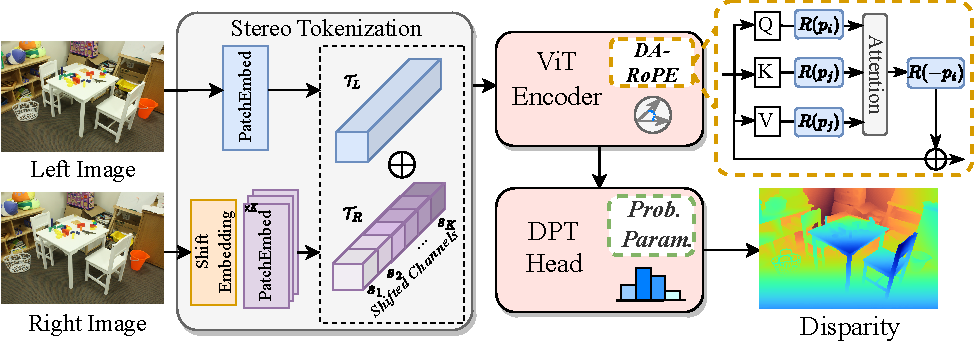
\includegraphics[width=0.98\linewidth]{fig/dispvit/method.pdf}
    \caption{\textbf{Overview of DispViT.}
    A rectified stereo pair is tokenized as a single binocular sequence.
    The resulting Transformer representation supports metric disparity decoding directly from the stereo-pair encoder.
    Stereo structure is preserved through tokenization and positional encoding rather than through an explicit cost volume.}
    \label{fig:dispvit_overview}
\end{figure}

\subsection{Shift-Embedding Stereo Tokenization}
\label{sec:dispvit_tokenizer}
The tokenizer must make a single-stream transformer compatible with epipolar geometry before any attention layer is applied.
A direct channel-wise concatenation of the left and right images would feed the patch embedding layer with pixels from identical image coordinates.
That assumption is poorly matched to rectified stereo, where the same 3D point may appear at a different horizontal location in the two views.
If patchification is performed before this displacement is considered, a token may already blend unrelated scene regions, leaving the transformer to undo a geometric error introduced at the input stage.

DispViT uses shift-embedding tokenization to expose coarse correspondence structure while keeping the representation single-stream.
Let $\mathcal{S}=\{s_1,\ldots,s_K\}$ be a set of horizontal offsets.
For each offset $s_k$, the right image is displaced along the epipolar direction and then embedded by a right-view branch $E^R_k$:
\begin{equation}
    \bm{T}^{R,k} = E^R_k\!\left(\operatorname{Shift}(\bm{I}^R,s_k)\right),
    \qquad k=1,\ldots,K .
    \label{eq:dispvit_shift_groups}
\end{equation}
For a Transformer token dimension $C$, each shifted right view is encoded into $C/K$ channels, and the $K$ shifted groups are concatenated along the channel dimension to recover a $C$-channel right-view token field.
This operation is implemented efficiently as a grouped convolution, so the shifted branches add geometric coverage without requiring $K$ independent full-width patch embeddings.
The token groups from the shifted right images are concatenated into the right-view contribution,
\begin{equation}
    \bm{T}^R = \operatorname{Concat}\!\left(\bm{T}^{R,1},\ldots,\bm{T}^{R,K}\right).
\end{equation}
The left image is embedded by a reference branch,
\begin{equation}
    \bm{T}^L = E^L(\bm{I}^L),
\end{equation}
and the two token fields are combined to form the binocular input sequence:
\begin{equation}
    \bm{T} = \bm{T}^L + \bm{T}^R .
    \label{eq:dispvit_token_blend}
\end{equation}

The shift-embedding tokenizer supplies geometric organization without becoming a cost volume.
It does not evaluate left-right representation similarity, store matching costs, or aggregate an explicit set of disparity hypotheses.
Instead, each token in the unified stereo-pair representation receives right-view evidence observed under several coarse horizontal offsets.
The transformer can then use attention to decide which displaced evidence is useful in context.
This design gives the unified representation early access to epipolar structure while avoiding a separate matching module.

\noindent\textbf{Asymmetric initialization.}
Pretrained patch embeddings are adapted to binocular input with an asymmetric initialization.
The left branch $E^L$ inherits the pretrained patch embedding weights, whereas the right-view shift branches are initialized to zero.
This choice keeps the reference-view appearance stable at the start of training and lets the right branches learn only the additional binocular evidence needed for disparity reasoning.
It also prevents the zero-initialized right-view branches from simply duplicating the left reference embedding, which helps the downstream Transformer distinguish reference appearance from displacement-specific binocular cues.

\subsection{Single-Stream Transformer Backbone}
The backbone is where DispViT deliberately brings semantic regularities and stereo evidence into one computation stream.
DispViT uses a Vision Transformer initialized from strong visual or depth-oriented pretraining, such as DINOv2~\cite{oquab2023dinov2} or Depth Anything V2~\cite{yang2024depth}.
The benefit is not limited to easier optimization.
Such pretraining gives the backbone access to object layout, scene structure, material appearance, and other visual regularities that are difficult to infer from local correspondence alone.
Stereo tokenization augments this pretrained visual representation with displacement cues from the right view, so the backbone can process semantic context and stereo geometry within one Transformer representation.
Thus, correspondence is no longer confined to a dedicated matching module; it becomes part of a global representation that can also encode semantic context.
This organization makes the backbone the main place where the thesis-level geometry-semantic representation is learned.

The Transformer output is decoded through multi-level representations in the style of DPT dense prediction heads~\cite{ranftl2021vision}.
Because left-view appearance and shifted right-view evidence have already been merged into a unified token field, each Transformer layer can propagate information across image regions while comparing candidate stereo alignments in context.
This global exchange is useful in regions where a local match is weak or misleading.
For instance, reflective or transparent surfaces may provide unreliable correspondence, but their boundaries, surrounding layout, and object category can still constrain plausible geometry.
The single-stream backbone is therefore used to make contextual scene understanding participate directly in metric disparity prediction.

\subsection{Semantic Readout as a Representation Probe}
\label{sec:dispvit_semantic_readout}
The semantic readout is a diagnostic probe for the unified representation rather than a second primary task.
Disparity remains the main geometric output of DispViT, but the thesis argument would be incomplete if the unified token space is evaluated only through depth accuracy.
A representation that truly combines semantic context with metric geometry should retain information about object categories, boundaries, and scene layout after it has been adapted to stereo input.
This chapter therefore attaches a lightweight semantic segmentation decoder to the representation used for disparity prediction.
Let $\bm{F}=\Phi_{\theta}(T_{\theta}(\bm{I}^L,\bm{I}^R))$ denote the unified stereo-pair representation.
The decoder $g_{\psi}$ maps this representation to a reference-view semantic prediction,
\begin{equation}
    \hat{\bm{S}} = g_{\psi}(\bm{F}),
    \label{eq:dispvit_semantic_readout}
\end{equation}
where $\hat{\bm{S}}$ assigns a semantic label to each pixel in the left image.

This decoder is intentionally used as a readout of representation content.
The central experiments still focus on disparity estimation, because stereo geometry is the main empirical setting of this chapter.
The segmentation probe complements those experiments by asking a different question: whether the stereo-pair representation preserves semantic structure while supporting metric disparity.
In the final thesis experiments, this component will be reported with standard semantic segmentation metrics such as mean Intersection-over-Union and pixel accuracy, and interpreted as evidence about the representation rather than as a competing segmentation model.

\subsection{Disparity-Aware Positional Encoding}
Positional encoding is the mechanism that gives spatial meaning to Transformer tokens.
Without it, self-attention can compare token content, but it has no explicit knowledge of where a patch lies or how two patches are displaced relative to one another.
For ordinary image recognition, encoding the absolute location of each patch is often sufficient.
However, stereo geometry imposes a stricter requirement: the model must reason about relative horizontal displacement, because in a rectified stereo pair this displacement is the geometric signal from which disparity is recovered.
Absolute position embeddings can mark where tokens are located, but they do not directly make token aggregation sensitive to the epipolar offset between a reference token and supporting evidence from nearby shifted tokens.

DispViT therefore introduces disparity-aware rotary positional encoding (DA-RoPE), an adaptation of rotary position embedding (RoPE) that makes relative displacement explicit inside the unified token space.
RoPE is a natural starting point because it expresses attention through relative offsets rather than only through absolute coordinates.
DispViT further applies the rotary transformation to value aggregation, so that information gathered by each query is expressed in the query token's local coordinate frame.
Let $p_i$ and $p_j$ denote token positions, $v_j$ the value vector at position $j$, and $\alpha_{ij}$ the attention weight from query $i$ to key $j$.
The resulting aggregation is
\begin{equation}
    \tilde{\bm{z}}_i
    =
    R(-p_i)\sum_j \alpha_{ij}R(p_j)\bm{v}_j
    =
    \sum_j \alpha_{ij}R(p_j-p_i)\bm{v}_j ,
    \label{eq:dispvit_darope}
\end{equation}
where $R(\cdot)$ denotes the rotary transformation, which rotates channel pairs in the value vectors by sinusoidal angles whose rates are determined by the RoPE frequency base.
Equation~\ref{eq:dispvit_darope} shows that each value contribution is modulated by the relative offset $p_j-p_i$.
This is important for stereo because the meaning of a visual cue depends on how it is displaced from the reference location, not merely on its absolute image coordinate.
The Transformer therefore receives an epipolar-compatible positional bias while preserving the global reasoning ability of self-attention.

DispViT further assigns different RoPE frequency bases to the horizontal and vertical axes.
In RoPE, a larger frequency base produces more slowly varying rotations, corresponding to longer positional wavelengths over which relative offsets remain distinguishable.
Because correspondence search in rectified stereo proceeds along the horizontal direction, DispViT uses a larger horizontal frequency base to extend positional sensitivity across distant columns.
This longer-range horizontal encoding is particularly beneficial for estimating large disparities, where corresponding points may be separated by many image tokens.
This design does not introduce an explicit cost volume or a separate matching pathway.
Instead, it makes metric displacement more legible inside the same representation that also carries semantic context, following the broader DispViT principle of injecting stereo geometry into a unified transformer stream.

\subsection{Probabilistic Disparity Regression}
\label{sec:dispvit_prob}
A unified representation still needs an output parameterization that is stable for dense metric geometry.
Regressing a single disparity value directly can be difficult because stereo targets cover a wide range and ambiguous regions may support several plausible depths.
DispViT therefore represents the output as a distribution over disparity bins before converting it to a continuous estimate.
Let $\{b_m\}_{m=1}^{M}$ denote uniformly sampled disparity bins and let $\bm{P}_{ij}\in\mathbb{R}^{M}$ be the predicted distribution at pixel $(i,j)$.
The continuous prediction is computed as an expectation over a local neighborhood around the most likely bin:
\begin{equation}
    \hat{D}_{0,ij} = \sum_{m \in \mathcal{N}(\arg\max \bm{P}_{ij})} \tilde{P}_{ijm} b_m ,
    \label{eq:dispvit_expectation}
\end{equation}
where $\tilde{P}_{ijm}$ is the normalized probability within the local window $\mathcal{N}(\cdot)$.
This parameterization keeps the global output space regularized like classification while preserving sub-bin precision through continuous decoding.
It also gives the model an explicit way to express uncertainty when several disparities remain plausible.

The disparity objective combines supervision on the binned distribution with supervision on the decoded metric value:
\begin{equation}
    \mathcal{L}_{\mathrm{reg}}
    =
    \operatorname{CE}\!\left(\bm{P},\operatorname{Bin}(D^{\ast})\right)
    +
    \lambda_1
    \left\lVert \hat{D}_0 - D^{\ast}\right\rVert_1 ,
    \label{eq:dispvit_loss}
\end{equation}
where $D^{\ast}$ is the ground-truth disparity and $\operatorname{Bin}(\cdot)$ converts each continuous target into a soft distribution over its two neighboring disparity bins.
Specifically, if $b_{\ell} \leq D^{\ast}_{ij} \leq b_{\ell+1}$, the lower and upper bins receive the linear interpolation weights $(b_{\ell+1}-D^{\ast}_{ij})/(b_{\ell+1}-b_{\ell})$ and $(D^{\ast}_{ij}-b_{\ell})/(b_{\ell+1}-b_{\ell})$, respectively, while all other bins receive zero weight.
The two nonzero weights sum to one and preserve the sub-bin location of the continuous target during classification-based supervision.
The cross-entropy (CE) term shapes the distribution over the full disparity range, while the $L_1$ term keeps the decoded estimate metrically accurate.

\subsection{Lightweight Local Refinement}
The direct DispViT prediction captures globally coherent geometry, but dense reconstruction also depends on fine spatial details that may be weakened during patch embedding and multi-scale decoding.
Thin structures, sharp object boundaries, and narrow depth discontinuities are particularly sensitive to this loss of spatial resolution.
DispViT therefore includes an optional lightweight refinement stage, adapted from NMRF~\cite{guan2024neural}, for applications that require higher local fidelity.

The refinement stage treats the initial disparity $\hat{D}_0$ as a geometric anchor rather than restarting stereo estimation from an unconstrained search space.
Using $\hat{D}_0$, right-view representations are warped toward the left reference view so that the remaining disagreement can be examined in an approximately aligned coordinate frame.
The refinement network then combines the aligned stereo evidence with fine-resolution image evidence and predicts a residual correction to the initial disparity.
Because the correction is conditioned on an already coherent estimate, the module can concentrate on local errors around boundaries and small structures instead of relearning the global scene geometry.

Keeping the refinement stage optional allows the standalone DispViT regressor to serve as a direct test of the chapter's central hypothesis: a unified geometry-semantic representation can support metric disparity without an explicit matching pipeline.
The refinement stage is then evaluated separately as a practical mechanism for restoring local precision; it neither introduces a full cost volume nor replaces the unified representation with iterative correspondence search.
Comparing the standalone and refined variants therefore distinguishes the geometry decoded through unified global reasoning from the additional accuracy contributed by task-specific local correction.
This separation provides a clearer attribution of performance gains while preserving the representation-learning role of DispViT.

\subsection{Training Strategy}
Training is organized to keep direct disparity regression and local refinement as two separate sources of improvement.
In the first stage, the stereo tokenizer, single-stream backbone, and probabilistic disparity head are jointly trained with the objective in Eq.~\ref{eq:dispvit_loss}.
At this point the model predicts only the initial disparity $\hat{D}_0$.
Its accuracy therefore reflects how much metric geometry can be recovered from the stereo-pair representation before any refinement network is allowed to correct local errors.

In the second stage, the trained regressor is frozen and only the optional refinement module is optimized.
The fixed prediction $\hat{D}_0$ provides the geometric initialization, and the refinement module learns residual corrections to produce the final disparity $\hat{D}$.
Because the tokenizer, backbone, and disparity head are no longer updated, the second stage cannot change the representation that produced $\hat{D}_0$; it can only improve local structures and boundaries on top of that estimate.
This staged protocol makes the experimental comparison interpretable: DispViT reports the direct output of the unified representation, whereas DispViT+ reports the additional gain from local refinement.

\section{Experiments}
\label{sec:dispvit_experiments}

\subsection{Evaluation Protocol}
The experiments are organized around three empirical questions that follow directly from the methodology.
First, can the unified binocular representation be decoded into accurate disparity without constructing an explicit cost volume?
Second, does the direct regressor remain reliable under domain shift and in regions where local matching is ambiguous?
Third, does the same unified representation preserve enough semantic information to support an auxiliary reference-view segmentation readout?
The first two questions are evaluated with standard stereo benchmarks, while the third is treated as a representation probe rather than as a standalone segmentation benchmark.

The stereo evaluation uses both synthetic and real-world data.
Scene Flow~\cite{mayer2016large} provides dense synthetic supervision for controlled quantitative comparison.
KITTI 2012~\cite{geiger2012we} and KITTI 2015~\cite{menze2015object} evaluate driving scenes with sparse LiDAR-based annotations.
Middlebury~\cite{scharstein2014high} and ETH3D~\cite{schops2017multi} stress cross-domain generalization through high-resolution indoor imagery, grayscale images, and low-texture regions.
The Booster dataset~\cite{zamaramirez2022booster} is used for qualitative analysis on transparent, reflective, and other matching-ambiguous materials.
The semantic readout is evaluated on reference-view segmentation annotations to test whether the representation produced from the stereo pair retains scene-level semantics.

The main metrics follow standard stereo evaluation practice.
End-point error (EPE) measures the mean absolute disparity error in pixels.
Bad-pixel rates (BP-$x$) report the percentage of pixels whose error exceeds a fixed threshold $x$.
For KITTI, the D1 metric counts pixels whose disparity error is both larger than 3 pixels and larger than 5 percent of the ground-truth disparity.
For semantic segmentation, the readout is evaluated with mean Intersection-over-Union and pixel accuracy.
Throughout the section, \emph{DispViT} denotes the standalone direct regressor, and \emph{DispViT+} denotes the variant with the lightweight refinement stage.

\subsection{Implementation Details}
\label{sec:dispvit_implementation}
Unless otherwise stated, the experiments use a ViT-L backbone initialized from Depth Anything V2~\cite{yang2024depth}.
The shift-embedding tokenizer uses $K=8$ horizontal shifts of the right image, with a 24-pixel interval between adjacent shifted views.
Following the channel allocation in Section~\ref{sec:dispvit_tokenizer}, each shifted right-view branch produces $C/K$ channels, and the shifted branches are concatenated along the channel dimension to form a $C$-channel token input.
The disparity head represents disparity with 128 uniformly spaced bins over the range $[0,381]$, and the loss in Eq.~\ref{eq:dispvit_loss} uses $\lambda_1=0.1$.
For DA-RoPE, the vertical and horizontal RoPE frequency bases are set to 100 and 1000, respectively, so the horizontal direction is assigned a longer positional wavelength for large-disparity reasoning.

All disparity models are trained with random image crops of size $392 \times 768$.
The direct regressor is pretrained on a mixed stereo corpus that includes FoundationStereo/FSD~\cite{wen2025foundationstereo}, Scene Flow~\cite{mayer2016large}, TartanAir~\cite{wang2020tartanair}, CREStereo~\cite{li2022practical}, InStereo2K~\cite{bao2020instereo2k}, FallingThings~\cite{tremblay2018falling}, Sintel~\cite{butler2012naturalistic}, and Virtual KITTI 2~\cite{cabon2020virtual}.
This pretraining mixture exposes the single-stream model to diverse disparity ranges, and rendering styles, before dataset-specific evaluation.
The optional refinement stage reuses the image encoder and refinement network from NMRF~\cite{guan2024neural}, but removes NMRF's disparity proposal network and multi-hypothesis inference so that the stage only learns residual local correction on top of $\hat{D}_0$.

For Scene Flow, evaluation follows the common protocol of considering only pixels whose ground-truth disparity is no larger than 192 pixels.
The pretrained direct regressor is fine-tuned on the Scene Flow training set, after which the refinement module is trained from scratch while the regressor remains frozen.
For KITTI benchmark evaluation, the pretrained regressor is kept frozen and only the refinement module is trained on the combined KITTI 2012 and KITTI 2015 training sets.
Because KITTI supervision is sparse and can be noisy near object boundaries, the refined KITTI variant uses two stacked refinement modules to give local correction more capacity.
The semantic readout is not part of the original disparity-training pipeline; it is evaluated separately in Section~\ref{sec:dispvit_semantic_experiments} as an auxiliary probe of the learned representation.

\begin{table}[!t]
    \centering
    \caption{\textbf{Scene Flow accuracy and runtime.}
    The standalone DispViT row evaluates the unified binocular representation before local refinement, while DispViT+ reports the additional gain from lightweight correction.
    Runtime is measured on an RTX 3090.}
    \label{tab:dispvit_sf_accuracy}
    \small
    \setlength{\tabcolsep}{6pt}
    \renewcommand{\arraystretch}{1.08}
    \vspace{-4pt}
    \begin{tabular*}{\textwidth}{@{\extracolsep{\fill}}llccc@{}}
        \toprule
        \textbf{Family} & \textbf{Method} & EPE $\downarrow$ & BP-1 $\downarrow$ & Time [s] \\
        \midrule
        \multirow{4}{*}{Matching} & RAFT-Stereo & 0.56 & 6.63 & 0.40 \\
        & DLNR & 0.48 & 5.39 & 0.33 \\
        & Selective-IGEV & 0.44 & 4.98 & 0.25 \\
        & NMRF & 0.45 & 4.50 & 0.10 \\
        \midrule
        \multirow{2}{*}{Hybrid} & DEFOM-Stereo & 0.42 & 5.10 & 0.63 \\
        & BridgeDepth & 0.37 & 3.67 & 0.14 \\
        \midrule
        \multirow{2}{*}{This chapter} & DispViT & 0.53 & 5.30 & 0.092 \\
        & DispViT+ & \textbf{0.34} & \textbf{3.50} & 0.118 \\
        \bottomrule
    \end{tabular*}
    \vspace{-4pt}
\end{table}

\subsection{Scene Flow Results}
Scene Flow provides a controlled testbed for assessing whether a single-stream Transformer can learn dense metric geometry from stereo pairs.
Because the dataset offers dense synthetic supervision over a wide range of scenes, it supports a direct comparison between DispViT, matching-centric stereo pipelines, and hybrid geometry-semantic methods under a common protocol.
In Table~\ref{tab:dispvit_sf_accuracy}, the standalone DispViT row is the primary evidence for the unified-representation claim, because it reports disparity decoded directly from the token representation produced from the stereo pair before the optional refinement stage.

Quantitatively, DispViT obtains 0.53 EPE and 5.30 BP-1 while running at 0.092 seconds per stereo pair.
Compared with RAFT-Stereo, it reduces EPE from 0.56 to 0.53 and BP-1 from 6.63 to 5.30, corresponding to relative reductions of 5.4\% and 20.1\%, respectively.
It is also about 4.3 times faster than RAFT-Stereo under the reported runtime setting.
DispViT does not yet match BridgeDepth in raw error, but this comparison should be read together with the architectural difference: BridgeDepth retains separate semantic and stereo pathways, whereas DispViT tests whether one Transformer stream can produce a useful geometric estimate directly.
The result therefore supports the thesis claim that a unified representation can encode metric geometry, while also showing where a dedicated two-pathway alignment pipeline can still be stronger before refinement.

DispViT+ measures how much residual improvement is available from local correction after the unified representation has produced its initial disparity.
It reduces EPE from 0.53 to 0.34 and BP-1 from 5.30 to 3.50, giving relative improvements of 35.8\% and 34.0\% over the direct regressor.
This gain adds 0.026 seconds over the standalone model, increasing runtime from 0.092 to 0.118 seconds.
The refined model still remains faster than BridgeDepth (0.118 versus 0.14 seconds) while improving both EPE and BP-1 (0.34/3.50 versus 0.37/3.67).
Because the direct regressor is frozen when training the refinement module, these numbers quantify the boundary and detail correction that can be added on top of the learned representation.
They do not shift the chapter's main evidence away from the standalone model; instead, they show that the unified representation provides a strong initialization that a lightweight local module can sharpen for benchmark fidelity.

\subsection{Zero-Shot Generalization}
Zero-shot generalization tests whether the learned binocular representation remains useful when the evaluation domain differs from the training data.
This setting is especially relevant to robotic perception, where deployment scenes may change in material, lighting, camera characteristics, and object composition.
Stereo systems that rely heavily on local texture matching can become brittle under such shifts because the most similar local patch may no longer correspond to the correct physical surface.
DispViT addresses this setting by decoding disparity from a representation that combines binocular evidence with semantic and structural context from large-scale pretraining.

\begin{table}[!t]
	\centering
	\small
	%\def\mywidth{0.47\textwidth} 
	%\tabcolsep=2.0pt
	%\resizebox{\mywidth}{!}{
		\begin{minipage}{0.59\textwidth}
			\centering
			\small
			\setlength{\tabcolsep}{3.0pt}
			\renewcommand{\arraystretch}{1.05}
			\vspace{-12pt}
			\caption{\textbf{Cross-dataset zero-shot evaluation.}
			Results use Scene Flow training unless marked by $^{\dagger}$ for additional stereo data.
			Middlebury (Q) is quarter-resolution; lower values are better.}
			\label{tab:dispvit_zero_shot}
			\vspace{2pt}
			\begin{tabular}{@{}lcccc@{}}
				\toprule
				\multirow{2}{*}{Method} & KITTI-12 & KITTI-15 & Middlebury (Q) & ETH3D\\
				& (D1) & (D1) & (BP-2) & (BP-1)\\
				\midrule
				%DSMNet & 6.2 & 6.5 & 8.1 & 6.2\\
				%Mask-CFNet & 4.8 & 5.8 & - & 5.7 \\
				
				%Former-RAFT-DAM & \cellcolor{yellow!25}3.9 & \cellcolor{yellow!25}5.1 & 5.4 & 3.3 \\
				%Training Set & \multicolumn{4}{c}{Scene Flow}\\
				%\midrule
				RAFT-Stereo & 4.7 & 5.5 & 9.4 & 3.3\\
				
				%IGEV-Stereo &5.2 & 5.7 & 8.8 & 4.0\\
				NMRF & 4.2 & 5.1 & 7.5 & 3.8\\
				IGEV++ & 5.1 & 5.9 & 7.8 & 4.1 \\
				DEFOM-Stereo & 3.8 & 5.0 & 5.7 & 2.4 \\
				%FoundationStereo~\cite{wen2025foundationstereo} & \cellcolor{red!25}\textbf{3.2} & \cellcolor{yellow!25}4.9 & \cellcolor{yellow!25}5.5 & \cellcolor{yellow!25}1.8 \\
				%\midrule
				BridgeDepth & 3.6 & 4.5 & 4.3 & 1.3\\
				%BridgeDepth (Mono$^\dag$) & 3.7 & 4.2 & 5.8 & 1.7\\
				Monster & 3.6 & 4.0 & 5.1 & 2.0\\
				Monster$^{\dagger}$ & 3.0 & 3.2 & 2.9 & 1.2\\
				%DEFOM & 3.8 & 5.0 & 3.3 & 2.4\\
				\midrule
				DispViT$^{\dagger}$ & 3.2 & 3.4 & 3.7 & 1.2\\
				DispViT+$^{\dagger}$ & 2.5 & 2.8 & 1.6 & 0.6\\
				\bottomrule
			\end{tabular}
				\vspace{-1.2em}
			\end{minipage}
			\hfill
			\begin{minipage}{0.39\textwidth}
				\centering
				\small
				\setlength{\tabcolsep}{4.5pt}
				\renewcommand{\arraystretch}{1.05}
				\caption{\textbf{ETH3D test-set leaderboard comparison.}
				DispViT+ achieves near-best AvgErr and the lowest RMSE among the listed methods on grayscale real-world stereo.}
				\label{tab:eth3d}
				\vspace{2pt}
				\begin{tabular}{@{}lcc@{}}
					\toprule
					\multirow{2}{*}{Method} & AvgErr & RMSE\\
				& (px) & (px)\\
				\midrule
				RAFT-Stereo   &  0.17 & 0.42\\
				Selective-IGEV   & 0.15 & 0.57\\
				IGEV++ & 0.19 & 0.74\\
				DEFOM-Stereo & 0.11 & 0.26\\
				BridgeDepth & 0.11 & 0.26\\
				Monster & 0.13 & 0.47\\
				FoundationStereo & 0.13 & 0.61\\
				\midrule
				DispViT+ & 0.12 & 0.25\\
				\bottomrule
			\end{tabular}
			\end{minipage}
		%\vspace{-10pt}
		\end{table}
	
Table~\ref{tab:dispvit_zero_shot} shows that the mixed-pretrained DispViT variants transfer strongly across driving, indoor, and grayscale reconstruction domains.
The direct DispViT regressor already improves over BridgeDepth on all four zero-shot settings, reducing the reported error from 3.6 to 3.2 on KITTI-12, from 4.5 to 3.4 on KITTI-15, from 4.3 to 3.7 on Middlebury, and from 1.3 to 1.2 on ETH3D.
After lightweight refinement, DispViT+ reaches 2.5/2.8 D1 on KITTI-12/15 and 1.6/0.6 BP on Middlebury/ETH3D.
Compared with Monster$^{\dagger}$, the strongest extra-data baseline in the table, DispViT+ reduces error by 16.7\% on KITTI-12, 12.5\% on KITTI-15, 44.8\% on Middlebury, and 50.0\% on ETH3D.
The ETH3D leaderboard results in Table~\ref{tab:eth3d} give a complementary test-set view: DispViT+ obtains 0.12 AvgErr and 0.25 RMSE, with AvgErr close to the best reported value of 0.11 and the lowest RMSE among the listed methods.

\begin{figure}
	\centering
	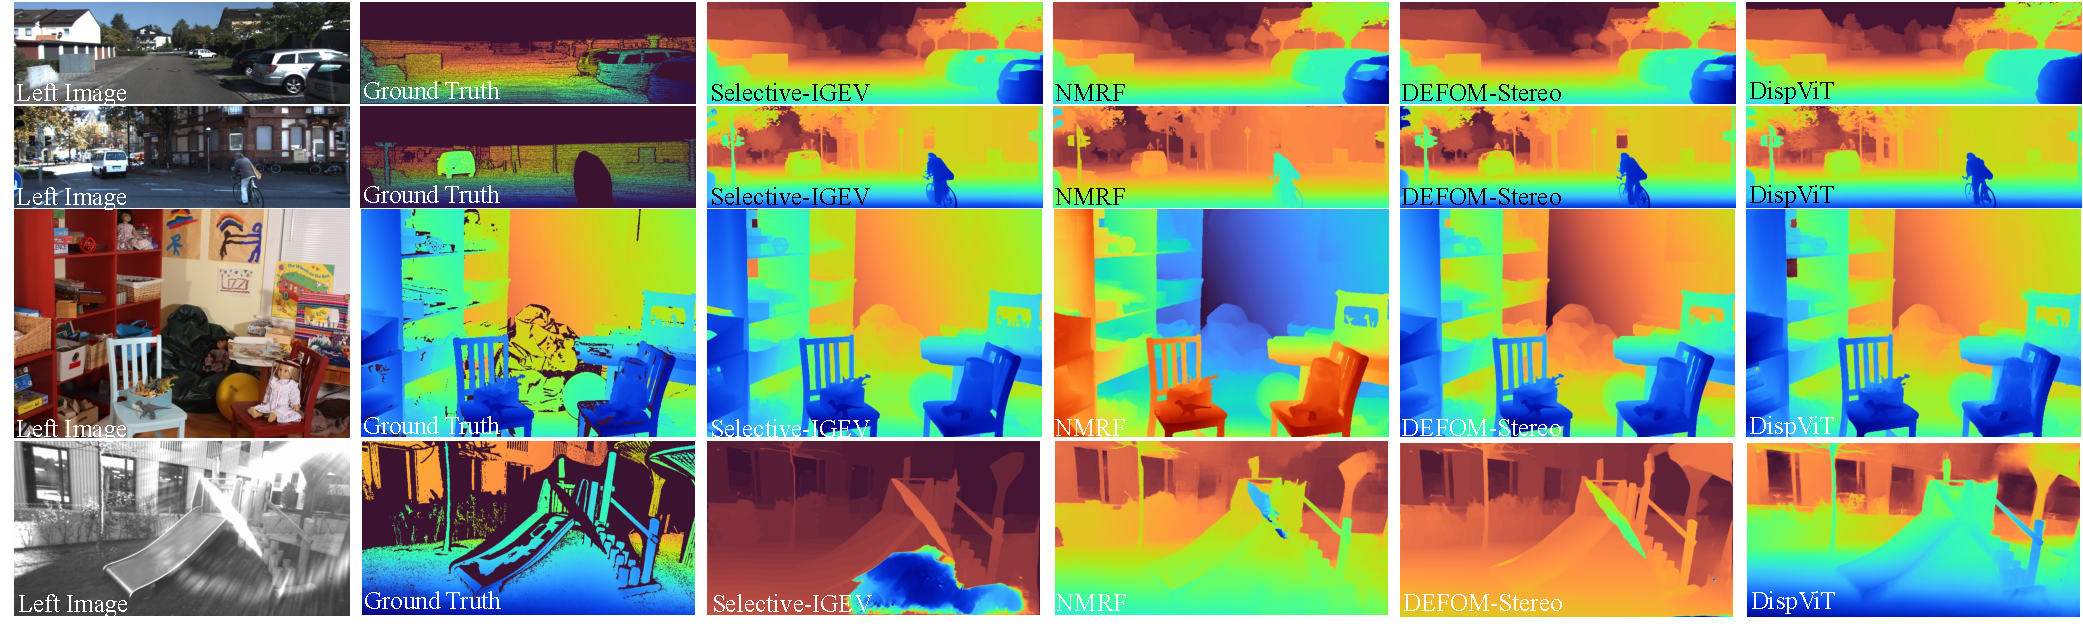
\includegraphics[width=0.98\linewidth]{fig/dispvit/zero_shot_black.pdf}
	\vspace{-6pt}
	\caption{\textbf{Qualitative zero-shot generalization across real-world datasets.}
	The examples compare DispViT with representative stereo baselines on scenes containing low texture, transparency, reflection, and other material-induced correspondence ambiguities.
	DispViT produces more coherent disparity in many regions where local matching becomes fragmented, supporting the role of global geometry-semantic context under domain shift.
	The remaining errors are most visible in mirror-like regions, where reflected scene content can be geometrically confused with the physical surface.}
	\vspace{-10pt}
	\label{fig:dispvit_zero_shot}
\end{figure}
			
The qualitative results are used to interpret why this transfer behavior differs from explicit local matching.
Matching-centric methods may perform well on ordinary textured surfaces, yet produce fragmented disparities on transparent, reflective, or low-texture regions whose appearance violates local matching assumptions.
DispViT reduces this type of local-correspondence failure by predicting from a global representation that can use surrounding layout, object boundaries, and learned scene priors when local evidence is weak.
The dominant residual failure observed in the qualitative examples is mirroring ambiguity.
In mirror-like or strongly reflective regions, the visible image evidence may correspond to reflected scene content rather than to the physical surface itself, so the global representation can still assign a coherent but incorrect disparity to the reflected structure.
This distinction is important for the thesis narrative: unified representations reduce isolated local mismatches, but they do not fully resolve cases where the image formation process makes the physical surface and the reflected scene geometrically ambiguous.

\subsection{KITTI and ETH3D Benchmarks}
KITTI and ETH3D evaluate whether the learned representation remains practical under benchmark protocols that differ from synthetic Scene Flow training.
KITTI focuses on outdoor driving scenes with large depth ranges, vehicles, thin structures, and frequent occlusions.
Its ground truth is derived from sparse LiDAR, so many pixels near object silhouettes and depth discontinuities are only partially observed.
This makes KITTI especially useful for testing whether the frozen unified regressor can provide a transferable geometric initialization while the refinement module adapts local boundaries and foreground objects.
ETH3D provides a complementary real-world test with grayscale images, fine structures, and many low-texture regions.
Strong ETH3D performance indicates that the representation is not tied only to color statistics or synthetic rendering appearance.
Together, KITTI and ETH3D separate two forms of transfer: benchmark adaptation to outdoor driving scenes and generalization to a visually different reconstruction setting.

\begin{table}[!t]
	\small
	\centering
	\caption{\textbf{KITTI 2012 and KITTI 2015 benchmark comparison.}
	KITTI 2012 reports Out-$x$, the percentage of pixels with disparity error larger than $x$ pixels, for non-occluded (Noc) and all pixels.
	KITTI 2015 reports D1 separately on background (BG) and foreground (FG) regions.
	Time$^\dag$ is measured on an RTX 3090, and lower values are better for all metrics.}
	\label{tab:dispvit_results_kitti}
	\vspace{6pt}
	\setlength{\tabcolsep}{8pt}
	\begin{tabular}{l c c c c c c c c c}
		
		\toprule
		& \multicolumn{4}{c}{KITTI 2012} & \multicolumn{4}{c}{KITTI 2015} &\\
		\cmidrule(lr){2-5}
		\cmidrule(lr){6-9}
		Method & \multicolumn{2}{c}{Out-2} & \multicolumn{2}{c}{Out-3}  
		& \multicolumn{2}{c}{BG} & \multicolumn{2}{c}{FG} & Time$^\dag$\\
		\cmidrule(lr){2-3}
		\cmidrule(lr){4-5}
		\cmidrule(lr){6-7}
		\cmidrule(lr){8-9}
		& Noc &  All &  Noc &  All & Noc & All & Noc & All & (s) \\
		%\cmidrule(lr){1-5}
		%\cmidrule(lr){7-10}
		\hline
		%GCNet~\cite{kendall2017end} & 16.58 & 19.07 & 10.80 & 12.80 & 2.71 & 3.46  & 1.77 & 2.30 &  2.21 & 6.16 &  2.87 & 0.9\\
		%PSMNet~\cite{chang2018pyramid} & 13.77 & 16.06 & 8.36 & 10.18 & 2.44 & 3.01 & 1.49 & 1.89  & 1.86 & 4.62 &  2.32 & 0.41\\  
		%GwcNet~\cite{guo2019group} & 12.49 & 14.57 & 7.80 & 9.28 & 2.16 & 2.71 & 1.32 & 1.70 & 1.74 & 3.93 & 2.11 & 0.32\\
		%GANet-deep  & 10.75 & 12.94 & 6.22 & 7.92 & 1.89 & 2.50 & 1.19 & 1.60 &1.48 &3.46 & 1.81 & - \\
		%CSPN & 10.40 & 12.73 & 6.40 & 8.17 & 1.79 & 2.27 & 1.19 & 1.53 & 1.51 & 2.88 & 1.74 & -\\
		
		LEAStereo & 1.90 & 2.39 & 1.13 & 1.45 & 1.29 & 1.40 & 2.65 & 2.91 & -\\
		PCWNet & 1.69 & 2.18 & 1.04 & 1.37 & 1.26 & 1.37 & 2.93 & 3.16 & -\\
		ACVNet & 1.83 & 2.35 & 1.13 & 1.47 & 1.26 & 1.37 & 2.84 & 3.07 & 0.2\\
		RAFT-Stereo & 1.92 & 2.42 & 1.30 & 1.66 & - & 1.58 & - & 3.05  & 0.38\\
		IGEV-Stereo & 1.71 & 2.17 & 1.12 & 1.44 & 1.27 & 1.38 & 2.62 & 2.67 & 0.18\\
		Selective-IGEV & 1.59 & 2.05 & 1.07 & 1.38 & 1.22 & 1.33 & 2.55 & 2.61 & 0.24 \\
		NMRF & 1.59 & 2.07 & 1.01 & 1.35 & 1.18 & 1.28 & 2.90 & 3.13 & \textbf{0.09}\\
		Mocha-Stereo & 1.64 & 2.07 & 1.06 & 1.36 & 1.24 & 1.36 & 2.42 & 2.43 & - \\
		
		
		%\cmidrule(lr){1-6}
		%\cmidrule(lr){7-10}
		%\hline
		%PBCP~\cite{seki2016patch} & 3.63 & 5.01 & 2.36 & 3.45 & 2.58 & 8.74 & 3.61 & 68\\
		%LBPS~\cite{knobelreiter2020belief} & - & - & - & - & 2.85 & 6.35 & 3.44 & 0.39\\
		\hline
		LoS & 1.69 & 2.12 & 1.10 & 1.38 & 1.29 & 1.42 & 2.66 & 2.81 & - \\
		MonSter & 1.36 & 1.75 & 0.84 & 1.09 & 1.05 & 1.13 & 2.76 & 2.81 & 0.45\\
		DEFOM-Stereo & 1.43 & 1.79 & 0.94 & 1.18 & 1.25 & 1.15 & \textbf{2.23} & \textbf{2.24} & 0.61\\
		%\hline
		IGEV++ & 1.36 & 1.74 & 0.89 & 1.13 & 1.07 & 2.80 & 2.80 & 2.80 & 0.48 \\
		BridgeDepth & 1.32 & 1.65 & 0.83 & 1.03 & 1.05 & 1.13 & 2.73 & 2.62& \textbf{0.14} \\
		\hline
		DispViT+ & \textbf{1.26} & \textbf{1.59} & \textbf{0.82} & \textbf{1.02} & \textbf{1.04} & \textbf{1.12} & 3.10 & 3.26 & 0.15\\
		\bottomrule
	\end{tabular}
	\vspace{5pt}
	%\vspace{-0.5em}
\end{table}

Table~\ref{tab:dispvit_results_kitti} shows that DispViT+ achieves the best KITTI 2012 results among the listed methods across both Out-2 and Out-3, for both non-occluded and all-pixel evaluations.
Relative to BridgeDepth, it reduces Out-2 All from 1.65 to 1.59 and Out-3 All from 1.03 to 1.02, while maintaining a comparable runtime of 0.15 seconds.
On KITTI 2015, DispViT+ obtains the best background D1 scores, 1.04 on non-occluded pixels and 1.12 on all pixels.
The foreground D1 scores, however, are weaker than the best foreground result in the table, with 3.10/3.26 compared with 2.23/2.24 from DEFOM-Stereo.
This pattern suggests that the unified representation transfers well to stable driving-scene geometry and background structure, while fast-moving or occluded foreground objects still place high demands on local boundary correction.
Together with the ETH3D leaderboard in Table~\ref{tab:eth3d}, where DispViT+ obtains 0.12 AvgErr and the lowest listed RMSE of 0.25, the benchmark results support the view that the representation is broadly transferable but still limited by difficult object-boundary.

\subsection{Semantic Segmentation Readout}
\label{sec:dispvit_semantic_experiments}
The semantic segmentation readout tests whether the DispViT representation obtained from binocular input contains semantic information that is not directly supervised by the disparity loss.
The experiment is not intended to turn DispViT into a segmentation system.
Instead, it freezes the disparity-trained encoder and asks whether a linear classifier can recover reference-view semantic labels from the token representation produced by the stereo pair.
The probe is evaluated in the reference-view coordinate frame because the disparity output is also defined on the left image, which keeps the geometric and semantic readouts on the same pixel grid.
For this readout, a $1 \times 1$ linear classifier is trained on Cityscapes~\cite{Cordts2016Cityscapes} training annotations using the concatenated patch tokens from the last four Transformer layers.
Because the backbone remains fixed, semantic accuracy reflects information already present in the representation learned from binocular input rather than adaptation of the encoder to segmentation.
Table~\ref{tab:semantic_linear_probe} compares DispViT with the original DINOv2~\cite{oquab2023dinov2} baseline under the same frozen-probe protocol on the Cityscapes validation set.

\begin{table}[!t]
    \centering
    \caption{\textbf{Cityscapes linear semantic probing from frozen representations.}
    A $1 \times 1$ classifier is trained on Cityscapes training annotations using concatenated last-four-layer patch tokens while the backbone remains fixed.
    Rows below the ``Per-class IoU'' divider report IoU for individual semantic classes.
    DINOv2 is evaluated with the same frozen-probe protocol; all values are percentages, and Gap denotes DispViT minus DINOv2.}
    \label{tab:semantic_linear_probe}
    \small
    \setlength{\tabcolsep}{6pt}
    \renewcommand{\arraystretch}{1.05}
    \begin{tabular*}{\textwidth}{@{\extracolsep{\fill}}llrrr@{}}
        \toprule
        \textbf{Group} & \textbf{Metric / Class} & \textbf{DispViT} & \textbf{DINOv2} & \textbf{Gap} \\
        \midrule
        Overall & mIoU & 58.59 & 74.29 & -15.70 \\
        Overall & Pixel Acc. & 93.63 & 94.78 & -1.15 \\
        Overall & Mean Acc. & 67.61 & 82.83 & -15.22 \\
        \midrule
        \multicolumn{5}{c}{\emph{Per-class IoU}} \\
        \midrule
        Stuff & road & 96.98 & 97.52 & -0.54 \\
        Stuff & building & 89.30 & 90.10 & -0.80 \\
        Stuff & vegetation & 89.77 & 89.48 & +0.29 \\
        Stuff & sky & 93.60 & 92.44 & +1.16 \\
        Stuff & sidewalk & 75.79 & 80.07 & -4.28 \\
        \midrule
        Common things & car & 88.46 & 93.75 & -5.30 \\
        Common things & person & 68.82 & 76.63 & -7.81 \\
        Common things & bicycle & 66.07 & 72.44 & -6.37 \\
        \midrule
        Rare things & rider & 27.38 & 56.27 & -28.89 \\
        Rare things & truck & 20.22 & 81.06 & -60.84 \\
        Rare things & bus & 37.36 & 87.48 & -50.12 \\
        Rare things & train & 22.89 & 79.30 & -56.40 \\
        Rare things & motorcycle & 33.44 & 65.19 & -31.75 \\
        \bottomrule
    \end{tabular*}
\end{table}

Table~\ref{tab:semantic_linear_probe} reveals a clear separation between scene layout and fine-grained category identity.
DispViT remains close to DINOv2 in overall pixel accuracy, with 93.63\% versus 94.78\%, and it performs strongly on several large stuff classes.
Road and building are within one percentage point of DINOv2, while vegetation and sky are slightly higher for DispViT.
These classes occupy broad regions and are closely tied to surface layout, so strong performance on them indicates that disparity training preserves semantic organization at the scale of scene structure.
The larger gap appears when the probe must separate object categories: DispViT trails DINOv2 by 15.70 points in mIoU and by 15.22 points in mean accuracy, with the largest drops on rare thing classes such as truck, bus, train, rider, and motorcycle.
Figure~\ref{fig:dispvit_cityscapes_class_frequency} explains why these rare thing classes are a useful stress test.
The classes that remain strong for DispViT, such as road, building, vegetation, and sky, occupy a large fraction of the annotated pixels.
In contrast, rider, truck, bus, train, and motorcycle appear much less frequently, so they test whether the frozen representation preserves fine-grained class identity beyond coarse scene layout.
Class frequency provides context rather than a complete explanation: DINOv2 is frozen and tested with the same linear-probe protocol, yet it retains much stronger rare-class separability.

\begin{figure}[!t]
    \centering
    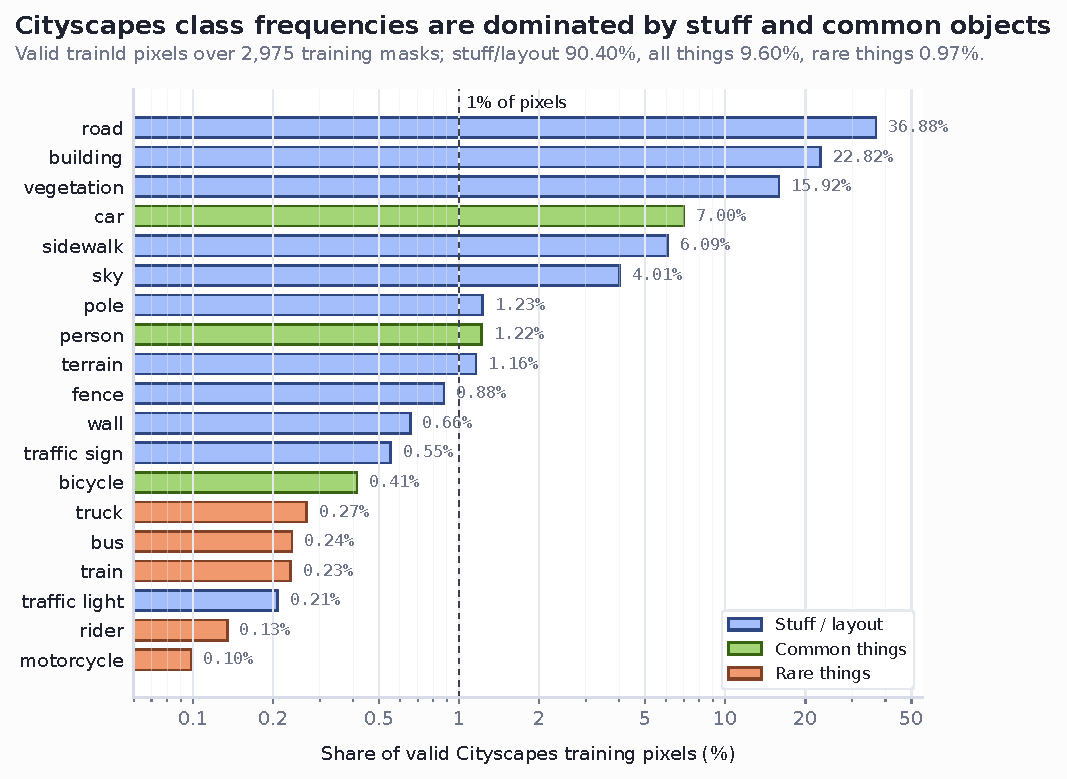
\includegraphics[width=0.94\linewidth]{fig/dispvit/cityscapes_class_frequency.pdf}
    \caption{\textbf{Cityscapes class-frequency distribution for semantic probing.}
    The distribution summarizes the semantic annotations used by the linear probe.
    Large stuff classes dominate the pixel count, while rare thing classes occupy substantially fewer pixels and therefore provide a sensitive test of fine-grained semantic separability.}
    \label{fig:dispvit_cityscapes_class_frequency}
\end{figure}

With this class-frequency context, the confusion matrices show what happens to the difficult thing-class pixels.
Table~\ref{tab:thing_error_aggregate} first aggregates all thing pixels and the rare thing subset for both frozen probes.
DispViT still recalls most thing pixels, with 86.90\% thing recall and only 5.52\% of thing pixels predicted as stuff.
The rare subset exposes the main limitation: rare thing recall drops to 34.75\%, and 41.74\% of rare-thing pixels are predicted as common thing classes.
Under the same probing protocol, DINOv2 reaches 84.05\% rare thing recall and only 7.99\% rare-to-common confusion.
Thus, the main semantic weakness of DispViT is not that objects are usually mistaken for background.
It is that rare object categories are often mapped to more common object categories.

\begin{table}[!t]
    \centering
    \caption{\textbf{Thing-class error decomposition for frozen Cityscapes linear probes.}
    All values are percentages.
    Rare things include rider, truck, bus, train, and motorcycle; common things include person, car, and bicycle.}
    \label{tab:thing_error_aggregate}
    \scriptsize
    \setlength{\tabcolsep}{3pt}
    \renewcommand{\arraystretch}{1.08}
    \begin{tabular*}{\textwidth}{@{\extracolsep{\fill}}lrrrrrrr@{}}
        \toprule
        \textbf{Model} &
        \makecell{\textbf{Thing}\\\textbf{recall}} &
        \makecell{\textbf{Thing}\\$\rightarrow$ \textbf{stuff}} &
        \makecell{\textbf{Thing}\\$\rightarrow$ \textbf{other thing}} &
        \makecell{\textbf{Rare}\\\textbf{recall}} &
        \makecell{\textbf{Rare}\\$\rightarrow$ \textbf{stuff}} &
        \makecell{\textbf{Rare}\\$\rightarrow$ \textbf{common thing}} &
        \makecell{\textbf{Rare}\\$\rightarrow$ \textbf{other rare}} \\
        \midrule
        DispViT & 86.90 & 5.52 & 7.58 & 34.75 & 15.74 & 41.74 & 7.77 \\
        DINOv2 & 93.08 & 4.63 & 2.29 & 84.05 & 7.18 & 7.99 & 0.78 \\
        \bottomrule
    \end{tabular*}
\end{table}

The class-level decomposition in Table~\ref{tab:dispvit_thing_confusion} makes this error mode concrete.
Trucks, buses, and trains are often predicted as cars; riders are frequently predicted as persons; and motorcycles are confused with bicycles or cars.
These mistakes suggest that the representation preserves coarse object grouping, but not all fine label distinctions required by semantic segmentation.
This behavior is consistent with supervision through the disparity loss alone: the encoder is rewarded for depth, object extent, and boundary placement, but it is not directly rewarded for separating different labels that can have similar 3D shape or occupy similar depth ranges.
The qualitative example in Figure~\ref{fig:dispvit_semantic_readout} shows the same pattern visually.
The frozen representation computed from the binocular input supports a coherent semantic layout, with the main scene structure and large regions recovered by the linear probe.
At the same time, person and rider regions can be confused even when the surrounding layout remains plausible.

\begin{table}[!t]
    \centering
    \caption{\textbf{Class-level thing errors for the DispViT semantic probe.}
    Percentages are computed over pixels of each ground-truth class.
    ``To stuff'' denotes predictions into Cityscapes stuff classes, while ``To other thing'' denotes predictions into another thing class; the last column reports the dominant wrong label and its percentage.}
    \label{tab:dispvit_thing_confusion}
    \small
    \setlength{\tabcolsep}{4pt}
    \renewcommand{\arraystretch}{1.05}
    \begin{tabular*}{\textwidth}{@{\extracolsep{\fill}}lrrrrl@{}}
        \toprule
        \textbf{GT class} & \textbf{IoU} & \textbf{Recall} & \textbf{To stuff} & \textbf{To other thing} & \textbf{Dominant error} \\
        \midrule
        person & 68.82 & 83.19 & 11.03 & 5.78 & building, 4.82 \\
        rider & 27.38 & 31.88 & 7.23 & 60.89 & person, 45.53 \\
        car & 88.46 & 97.05 & 2.15 & 0.80 & road, 0.79 \\
        truck & 20.22 & 22.90 & 26.76 & 50.34 & car, 43.51 \\
        bus & 37.36 & 43.15 & 12.03 & 44.83 & car, 34.91 \\
        train & 22.89 & 38.72 & 20.45 & 40.83 & car, 20.21; bus, 19.94 \\
        motorcycle & 33.44 & 40.73 & 8.51 & 50.76 & bicycle, 17.76 \\
        bicycle & 66.07 & 81.06 & 10.63 & 8.31 & person, 3.22 \\
        \bottomrule
    \end{tabular*}
\end{table}

\begin{figure}[!t]
    \centering
    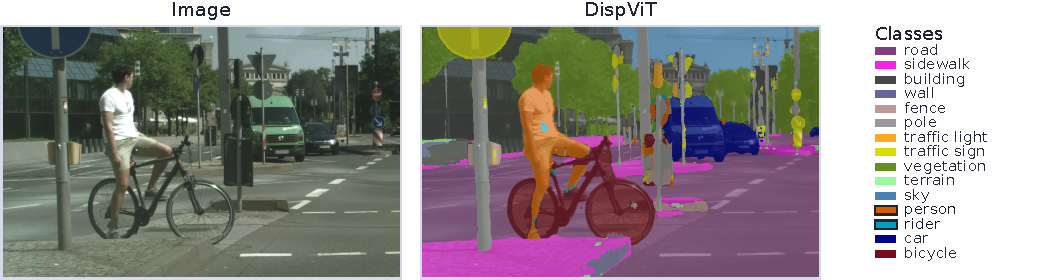
\includegraphics[width=0.94\linewidth]{fig/dispvit/semantic_single_dispvit.pdf}
    \caption{\textbf{Qualitative semantic readout from DispViT.}
    The linear probe recovers the dominant scene layout and broad semantic structure from the frozen DispViT representation produced by binocular input.
    The example also shows the main limitation identified by the quantitative analysis: fine-grained thing distinctions, such as person--rider separation, remain ambiguous.}
    \label{fig:dispvit_semantic_readout}
\end{figure}

Taken together, these results support a careful version of the unified-representation claim.
DispViT is not merely a disparity regressor, because one encoder can map binocular input to a representation that retains metric structure, object grouping, and scene-level semantic organization.
However, disparity supervision alone does not provide enough category-level signal for high-quality semantic segmentation, especially for rare object identities.
Additional semantic alignment or multi-task supervision would be needed if the encoder were expected to support both dense disparity and fine-grained semantic parsing directly.

\subsection{Ablation Studies}
The ablation studies test which design choices make single-stream regression trainable and accurate.
This analysis is important because the high-level architecture is deliberately simple: the stereo pair is mapped into one token stream and decoded directly.
Without the supporting geometric biases, this formulation may lose the structure needed for reliable disparity estimation.
The ablations therefore ask how much stereo geometry must be built into the tokenizer, positional encoding, and output parameterization for the unified representation to work.

\begin{table}[!t]
    \centering
    \caption{\textbf{Component analysis for direct disparity regression.}
    Removal studies ablate one design choice from the baseline regressor, while addition studies accumulate stereo-aware components.
    Lower EPE and BP-1 indicate more accurate disparity.}
    \label{tab:dispvit_abl}
    \small
    \setlength{\tabcolsep}{10pt}
    \renewcommand{\arraystretch}{1.12}
    \begin{tabular}{@{}lrrr@{}}
        \toprule
        \textbf{Variant} & \textbf{EPE $\downarrow$} & \textbf{BP-1 $\downarrow$} & \textbf{Time [s]} \\
        \midrule
        \multicolumn{4}{@{}l}{\emph{Removal studies from the baseline}} \\
        \addlinespace[1pt]
        Baseline (ViT-B) & 0.89 & 10.05 & 0.039 \\
        \quad No DAv2, scratch init & 1.81 & 20.13 & 0.039 \\
        \quad No DAv2, DINOv2 init & 0.92 & 10.79 & 0.039 \\
        \quad No probabilistic head & 1.07 & 15.56 & 0.027 \\
        \quad No asymmetric init & 0.97 & 11.88 & 0.039 \\
        \quad No RoPE, using APE & 0.96 & 13.34 & 0.042 \\
        \midrule
        \multicolumn{4}{@{}l}{\emph{Cumulative addition studies}} \\
        \addlinespace[1pt]
        Baseline + SE & 0.84 & 9.22 & 0.040 \\
        Baseline + SE + DA & 0.82 & 8.84 & 0.042 \\
        Baseline + SE + DA + AF & 0.76 & 8.27 & 0.042 \\
        \bottomrule
    \end{tabular}
\end{table}

Table~\ref{tab:dispvit_abl} separates the ablation evidence into removal and cumulative-addition studies.
The removal block shows that pretraining is the largest stability factor: training the ViT-B regressor from scratch raises EPE from 0.89 to 1.81 and nearly doubles BP-1 from 10.05 to 20.13.
Replacing Depth Anything V2 initialization with DINOv2 is much less damaging, but still slightly weakens the baseline, suggesting that depth-oriented pretraining better matches the metric geometry readout.
The probabilistic head is also important: removing it increases EPE to 1.07 and BP-1 to 15.56.
The bin-based head supervises a distribution over nearby disparity hypotheses before decoding a continuous value, whereas a single-value head must learn the full disparity scale from one continuous target per pixel.
Asymmetric initialization and RoPE provide smaller but consistent gains, supporting the need for a stable reference-view branch and offset-aware positional bias.

The cumulative addition block clarifies how stereo-aware biases improve the direct regressor.
Adding shift-embedding reduces EPE from 0.89 to 0.84, showing that coarse horizontal offsets help the single-stream tokenizer before attention begins.
Adding DA-RoPE further lowers EPE to 0.82 by making value aggregation sensitive to relative stereo displacement.
The asymmetric horizontal frequency design gives the strongest result in the table, 0.76 EPE and 8.27 BP-1, indicating that long-range horizontal sensitivity is especially useful for the epipolar structure of rectified stereo.
Figure~\ref{fig:dispvit_range_ablation} breaks down these effects by disparity interval.
Together, these ablations connect the empirical results back to the chapter's main claim: a single representation can carry semantic context and metric geometry, but it becomes more reliable when lightweight geometric biases make binocular displacement legible to the transformer.

\begin{figure}[!t]
    \centering
    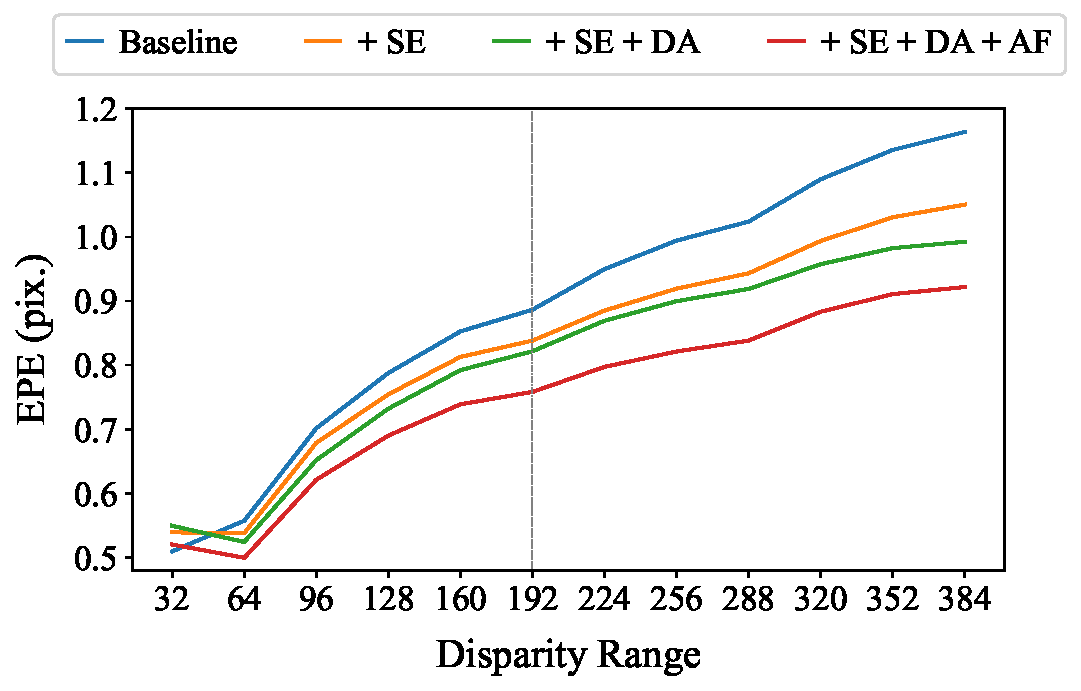
\includegraphics[width=0.62\linewidth]{fig/dispvit/abla_compare_disprange.pdf}
    \vspace{-5pt}
    \caption{\textbf{Disparity-range analysis of stereo-aware components.}
    End-point error is reported over different disparity intervals to show where each geometric bias contributes.
    Shift-embedding (SE) and DA-RoPE (DA) reduce errors most clearly in large-disparity regions, where pre-attention misalignment and long horizontal offsets are more severe.
    Asymmetric horizontal frequency further improves the curve across ranges by making the positional encoding more compatible with epipolar displacement.}
    \label{fig:dispvit_range_ablation}
\end{figure}

\subsection{Ambiguous Materials and Failure Cases}
Ambiguous materials provide a qualitative stress test for the binocular representation learned by DispViT.
Transparent, reflective, low-texture, and mirror-like regions are difficult for stereo because the visible image evidence may not correspond cleanly to the physical surface that should receive the disparity label.
Figure~\ref{fig:dispvit_booster} evaluates this behavior on challenging Booster examples~\cite{zamaramirez2022booster}.
The pretrained model is often able to recover plausible geometry on transparency, weak texture, and reflections, suggesting that the single-stream representation can use broader scene context when local matching evidence is unreliable.
The main remaining failure mode is mirroring ambiguity.
When a mirror produces a coherent reflected scene, the binocular cues can support a visually plausible but physically incorrect surface interpretation.
This boundary is important for the thesis: unified representation learning improves the use of context, but it does not remove the need for stronger priors about optical materials and physical surfaces.

\begin{figure}[!t]
    \centering
    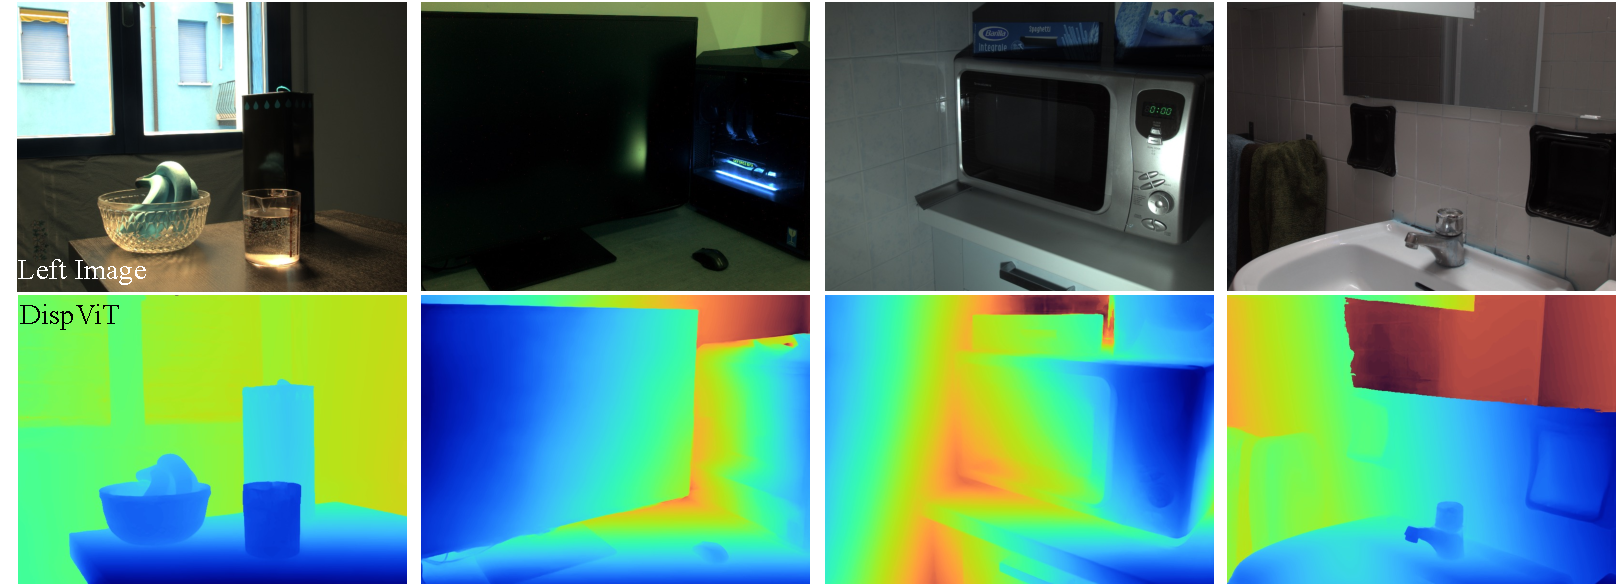
\includegraphics[width=0.98\linewidth]{fig/dispvit/booster.pdf}
    \caption{\textbf{Qualitative Booster results on matching-ambiguous materials.}
    The examples include transparent, low-texture, reflective, and mirror-like regions where local correspondence can be unreliable.
    DispViT often recovers plausible disparity by decoding geometry from a binocular representation that also carries scene context.
    The mirror example illustrates a remaining limitation: reflected content can create a coherent but incorrect geometric explanation, leaving mirroring ambiguity unresolved.}
    \label{fig:dispvit_booster}
\end{figure}

\section{Discussion}
\label{sec:dispvit_discussion}

\subsection{Relation to BridgeDepth}
The transition from BridgeDepth to DispViT is a transition from alignment to unification.
BridgeDepth begins with two specialized forms of evidence: monocular context and stereo hypotheses.
Its contribution is to let them exchange information through bidirectional latent interaction before the final prediction.
DispViT starts from a different assumption.
Rather than maintaining separate streams and aligning them later, it constructs one token representation from the stereo pair and lets the transformer learn semantic context and binocular geometry together.

This distinction matters for the thesis argument.
BridgeDepth demonstrates that monocular semantic priors and stereo geometric evidence should influence each other during inference.
DispViT pushes this interaction earlier, at the level where the representation itself is formed from binocular input.
The resulting token representation can support metric disparity decoding and can also be probed for reference-view semantic segmentation.
In this sense, DispViT moves closer to the kind of representation that a robotic perception system may need: not isolated estimators for geometry and semantics, but one visual representation from which both kinds of judgment can be read.

\subsection{Why Unified Regression Can Improve Robustness}
The robustness of DispViT comes from changing where ambiguous evidence is resolved.
In matching-centric pipelines, a cost volume or correlation module often commits early to a set of local correspondence scores.
If a textureless wall, glass panel, repeated pattern, or reflective surface produces misleading evidence, the matching representation may already favor the wrong disparity before broader context can correct it.
DispViT delays this commitment by first building a transformer representation from the binocular input.
The disparity head then decodes geometry after the representation has combined coarse epipolar alignment, semantic context, and long-range spatial information.

This does not mean that DispViT discards stereo geometry.
The model is still constrained by rectified binocular input, shift-embedding tokenization, DA-RoPE, and supervised metric disparity.
The difference is that geometric cues are embedded into a representation that can also carry scene-level regularities.
Precise binocular evidence remains useful where correspondence is reliable, while semantic and structural context can help in regions where local matching is weak.
This balance is the direction pursued throughout the thesis: robust depth perception emerges when geometric constraints and learned context are treated as mutually informative signals inside the same inference.

\subsection{Implications for Robotic Perception}
For robotics, the significance of DispViT lies beyond stereo benchmark accuracy.
A robot operating in the real world must reason about both where surfaces are and what those surfaces mean for action.
Depth supports obstacle avoidance, grasp planning, locomotion, and mapping.
Semantics supports object interaction, affordance reasoning, and scene-level decision making.
If these forms of information are produced by isolated modules, downstream systems must reconcile predictions that may disagree near object boundaries, reflective surfaces, or rare categories.
Unified representations offer a more integrated alternative: a perception backbone whose internal state already encodes metric structure and semantic organization.

DispViT is one step in this direction for rectified stereo.
Disparity remains the main output and the dominant experimental focus, but the semantic readout shows that the representation produced from binocular input also preserves scene-level semantic organization.
This is compatible with broader geometry foundation models that predict depth, point maps, camera parameters, and correspondences from general visual input~\cite{wang2025vggt}.
The contribution of this chapter is narrower but complementary: it shows that even the classical stereo problem can be reframed as transformer representation learning, rather than only as explicit correspondence search.

\subsection{Limitations}
DispViT also has clear limitations.
First, the current formulation depends on rectified stereo input and supervised disparity data.
The representation is learned primarily through binocular disparity estimation, and semantic segmentation is used as an auxiliary probe rather than as a jointly optimized task.
Second, the semantic readout shows strong scene-layout information but weaker rare-object separability.
This means that geometry supervision alone is not enough when the target application requires fine-grained semantic parsing.
Third, the Booster examples show that mirror-induced appearances can still mislead the model.
When reflected content forms a coherent false scene, binocular evidence and contextual reasoning may agree on the wrong physical surface.
Fourth, the optional refinement stage reintroduces local correction for high-frequency details.
This is useful for benchmark fidelity, but it also shows that direct global regression does not fully replace fine-scale geometric refinement.
Finally, the large transformer backbone increases memory and computation compared with compact stereo networks, although avoiding a full cost volume and iterative matching helps maintain practical efficiency.

These limitations suggest several directions for future work.
Scaling stereo pretraining with more diverse real and synthetic binocular data could improve robustness under distribution shift.
Adding semantic supervision or distilling semantic geometry priors from monocular models could improve rare-object separability and help with reflective or transparent surfaces.
Extending the single-stream formulation beyond rectified pairs toward multi-view or temporal input would also connect naturally to the next part of the thesis, where motion cues provide another source of geometric evidence.

\section{Conclusion}
\label{sec:dispvit_conclusion}
This chapter presented DispViT as a step toward unified geometry-semantic representation learning from stereo input.
The chapter reframed stereo from explicit correspondence search into direct decoding from a transformer representation produced by a binocular pair.
Shift-embedding tokenization, asymmetric stereo initialization, DA-RoPE, and probabilistic disparity prediction make this single-stream formulation trainable and accurate without constructing a full cost volume.
The main evidence comes from disparity estimation, where the standalone regressor validates that metric geometry can be decoded from the learned representation and the optional refinement stage restores fine local detail.
The semantic readout adds a complementary test: the frozen representation preserves scene layout and object grouping, although rare-object separability remains limited.

Within the thesis, DispViT advances the narrative from BridgeDepth's two-pathway latent alignment toward unified representation learning.
BridgeDepth showed that monocular priors and stereo hypotheses should interact.
DispViT shows that a single transformer stream can internalize semantic context and binocular geometry from the start.
The chapter therefore supports the broader thesis hypothesis that robotic perception will benefit from visual representations in which 3D geometry and semantic understanding are learned together, rather than fused only after separate estimation pipelines have already made their predictions.
